\iffalse
	前言:
		参考自一个祖传的模板,以及https://github.com/LeyuDame/BNUCV/tree/main 上的BNU的latex简历模板中的代码。
		注意要用XeLaTeX编译链进行编译,且要进行三次编译才能显示照片。问就是LaTeX的锅。
		vscode+latex的话,配置的json中"latex-workshop.latex.recipes"添加:
		{
            "name": "XeLaTeX*3",
            "tools": [
                "xelatex",
                "xelatex",
                "xelatex"
            ]
        }
		即可使用三次XeLaTeX编译。

		LaTeX+VScode怎么配置看https://www.zhihu.com/column/p/166523064。

        每个章节的格式都能混着用,顺序都可以变,只是给了个例子。
        比如你找工作,可以把技能那部分往前挪。
        比如你竞赛经历很多,你就往前挪。
        比如你觉得“其他”有点多余,就删了。

        主要贡献还是把原本word的那个模板页眉页脚和背景完美加进来了。
        LaTeX排版就是很整齐,强迫症狂喜。


        然后就是更新之后就不需要手动为每一页添加页脚页眉背景了,也不用newnewpage了,用一个bug解决了另一个bug。

        记得要三次XeLaTeX编译!!!
        记得要三次XeLaTeX编译!!!
        记得要三次XeLaTeX编译!!!
        这个很重要,所以说三遍!
        可以试试两次的,好像某些环境两次编译也能显示图像,但最好还是三次编译。
\fi

\documentclass[11pt]{article}
\usepackage{tikz}
\usetikzlibrary{calc}
\usepackage{xltxtra}
\usepackage{bookmark}
\usepackage{hyperref}
\hypersetup{hidelinks}
\usepackage{url}
\urlstyle{tt}
\usepackage{multicol}
\usepackage{xcolor}
\usepackage{calc}
\usepackage{graphicx}
\usepackage{fontspec}
\usepackage{xeCJK}
\usepackage{relsize}
\usepackage{xspace}
\usepackage{fontawesome}
\usepackage{titlesec}
\usepackage{enumitem}
\usepackage{siunitx}
\usepackage{amssymb}
\usepackage{tabularx}
\usepackage{multicol}
\usepackage{fontspec}
\usepackage{caption}
\usepackage{everypage}
\usepackage{enumitem} 

%%%%%%%%%%%%%%%%%%%%%%%%%%%%%%%%%%%%%%%%%%%%%%%%%%%%%%%%%%%%%%%%%
%							记得改这里							%
%%%%%%%%%%%%%%%%%%%%%%%%%%%%%%%%%%%%%%%%%%%%%%%%%%%%%%%%%%%%%%%%% 
% 学院
\newcommand{\configSchool}{计算机学院 | School of Computer And Science}
% 也可以不写英语
%\newcommand{\school}{电子信息学院}
% 联系方式

%%%%%%%%%%%%%%%%%%%%%%%%%%%%%%%%%%%%%%%%%%%%%%%%%%%%%%%%%%%%%%%%%
%							页面设置							%
%%%%%%%%%%%%%%%%%%%%%%%%%%%%%%%%%%%%%%%%%%%%%%%%%%%%%%%%%%%%%%%%% 
% 页面大小与页边距,按需求调整
\usepackage[
	a4paper,
	left=1.2cm,
	right=1.2cm,
	top=1.5cm,
	bottom=0cm,
	nohead
]{geometry}

% 每页自动添加背景,页眉,页脚,bug已解决
\AddEverypageHook{
    \begin{tikzpicture}[remember picture, overlay]
        % 背景
		\node[opacity=0.05](background) at(current page.center){
			
\includegraphics[width=0.7\paperwidth, keepaspectratio]{images/npu_logo_big.png}
		};
        % 页眉
        \node[anchor=north, inner sep=0pt](header) at (current page.north){
			
\includegraphics[width=\paperwidth]{images/header.png}
		};
        % 校徽
		\node[anchor=west](school_logo) at (header.west){
			\hspace{0.5cm}
			
\includegraphics[width=0.25\textwidth]{images/npu_logo_2.png}
		};
        % 学院名
		\node[anchor=east](school_name) at(header.east){
			\textcolor{white}{\textbf{\configSchool}}
			\hspace{0.5cm}
		};
        % 页脚
        \node[anchor=south, inner sep=0pt](footer) at (current page.south){
			
\includegraphics[width=\paperwidth]{images/footer.png}
		};
        % 联系方式
        %\node[anchor=center] at(footer.center){\configContact};
    \end{tikzpicture}
}

%%%%%%%%%%%%%%%%%%%%%%%%%%%%%%%%%%%%%%%%%%%%%%%%%%%%%%%%%%%%%%%%%
%							字体设置							%
%%%%%%%%%%%%%%%%%%%%%%%%%%%%%%%%%%%%%%%%%%%%%%%%%%%%%%%%%%%%%%%%% 
% 英文字体
\setmainfont[
    Path=fonts/,
    Extension=.ttf,
    BoldFont=* Bold,
]{Microsoft Yahei}
% 中文字体
\setCJKmainfont[
    Path=fonts/,
    Extension=.ttf,
    BoldFont=* Bold,
]{Microsoft Yahei}

%%%%%%%%%%%%%%%%%%%%%%%%%%%%%%%%%%%%%%%%%%%%%%%%%%%%%%%%%%%%%%%%%
%							样式设置							%
%%%%%%%%%%%%%%%%%%%%%%%%%%%%%%%%%%%%%%%%%%%%%%%%%%%%%%%%%%%%%%%%%
% 一级标题
\titleformat{\section}					    % 将原标题前面的数字取消了
  {\Large\bfseries\raggedright} 		    % 字体改为LARGE,bold,左对齐
  {}{0em}                      			    % 可用于添加全局标题前缀
  {}                           			    % 可用于添加代码
  [{\color{NPU_Blue}\titlerule}]            % 标题下方加一条线
\titlespacing*{\section}{0cm}{*0.5}{*0.5}	% 标题左边留白,上方1.2倍,下方1.2倍

% 二级标题
\titleformat{\subsection}				    % 将原二级标题前面的数字取消了
  {\large\bfseries\raggedright} 		    % 字体改为large,bold,左对齐
  {}{0em}                      			    % 可用于添加全局二级标题前缀
  {}                           			    % 可用于添加代码
  []
\titlespacing*{\subsection}{0cm}{*1}{*1}% 二级标题左边留白,上方1.2倍,下方1.2倍

% 图例的caption格式设置
\captionsetup[figure]{
    labelfont={},
    labelformat={default},
    labelsep=period,name={图}               % 这里表示你的caption会以“图1”,“图2”,“图3”开头,可以自行更换前缀
}

\CJKsetecglue{}							            % 取消中文字符与数字之间的间隔
\setlength{\parindent}{0pt}							% 取消全局段落缩进
\pagenumbering{gobble}								% 取消页码显示

% 这是个更好看的C++写法,你直接写C++的话,+号会很大,可以使用\Cpp来代替
\protected\def\Cpp{{C\nolinebreak[4]\hspace{-.05em}\raisebox{.28ex}{\relsize{-1}++}}\xspace}
% 中文字符间距
\renewcommand{\CJKglue}{\hskip 0.05em}
% 这里把表格的行间距调成1.2倍了
\renewcommand{\arraystretch}{1.1}
% 这里把正文的行间距调成1.2倍了
\linespread{1.2}

% 主题色
% 西工大蓝
\definecolor{NPU_Blue}{RGB}{0, 80, 158}

\setlength{\leftmargini}{9pt}  % 调整第一级 itemize 缩进

%%%%%%%%%%%%%%%%%%%%%%%%%%%%%%%%%%%%%%%%%%%%%%%%%%%%%%%%%%%%%%%%%
%							正文开始							%
%%%%%%%%%%%%%%%%%%%%%%%%%%%%%%%%%%%%%%%%%%%%%%%%%%%%%%%%%%%%%%%%%
\begin{document}

    %%%%%%%%%%%%%%%% 这段别删,这个段莫名其妙解决了一个大bug %%%%%%%%%%%%%%%%
        % 原本XeLaTeX好像和tikz有一点不兼容
        % 如果直接使用background包或者AddEverypageHook的话,第一页的透明度会失效,会很丑
        % 仿佛就像透明度相关的引擎没启动一样
        % 但是莫名其妙的加上这段之后
        % 莫名其妙又好了
        % 你可以删了看看效果
    \begin{tikzpicture}[remember picture, overlay]
        % 注意这里opacity=0不要改,这里主要是启动了tikz的透明度功能
        \node[opacity=0](background) at(current page.center){
            
\includegraphics[width=0.7\paperwidth, keepaspectratio]{images/npu_logo_big.png}
        };
    \end{tikzpicture}
    %%%%%%%%%%%%%%%% 这段别删,这个段莫名其妙解决了一个大bug %%%%%%%%%%%%%%%%

    \vspace{-2.03em}      
	% 个人信息
    \begin{figure}[h]
        % 左半边,信息,比例占行宽87%,可以自己调
        \begin{minipage}{0.85\textwidth}
            \section{\makebox[\widthof{\faUser}][c]{\color{NPU_Blue}{\faUser}}\quad \hspace{0.1em} 个人信息}
            %\small
            \begin{tabularx}{\linewidth}{p{\widthof{出生日期:}}Xp{\widthof{政治面貌:}}X}
                姓名: & 杨浩森 & 性别: & 男 \\
                出生日期: & 2003年11月18日 & 政治面貌: & 共青团员 \\
                联系邮箱: & 1961335143@qq.com &生源地: &山东德州
            \end{tabularx}
        \end{minipage}
        % images/example_avatar.png 替换成你证件照的路径。
        \begin{minipage}{0.14\textwidth}
            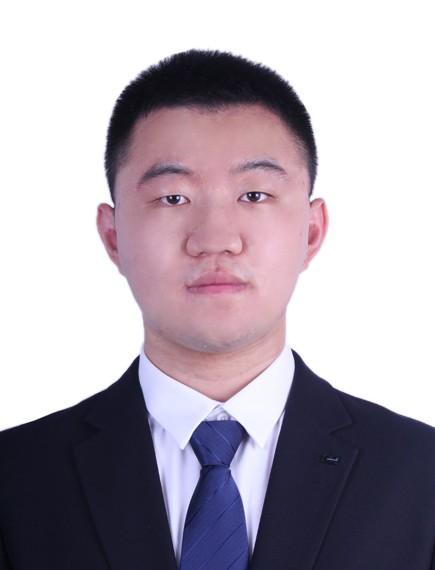
\includegraphics[width=\linewidth]{images/example_yang.jpg}
        \end{minipage}
        % 尽量留至少1%的间距,不然会换行
    \end{figure}

    \vspace{-2.5em} 
    
    %第二部分 教育背景 	
    \section{\makebox[\widthof{\faGraduationCap}][c]{\color{NPU_Blue}{\faGraduationCap}}\quad 教育背景}
        \subsection{2021.09-2025.07\hfill 西北工业大学 \hfill 计算机科学与技术(本科)}
        \vspace{-0.2em}
    
        \begin{itemize}
        \setlength{\itemsep}{0pt}  % 设置列表项间距为 0
        \setlength{\parsep}{0pt}   % 设置段落间距为 0
        \setlength{\parskip}{0pt}  % 设置段后额外间距为 0
        \item\textbf{主修课程及成绩:} 计算机组成与系统结构(98),数据库原理实验(100),人工智能芯片设计导论(96),高级语言程序设计实验(99),神经网络模型与算法(95),程序设计基础实验(97),高级语言程序设计(92),信号与系统实验(96),统计计算语言学(90),软件工程实验(93)等。
        \item\textbf{荣誉奖励:} 陕西省第十三次大学生高等数学(本科)竞赛二等奖;2022-2023年优秀大学生、学业先进个人,程序设计实验技能竞赛一等奖(2022)、二等奖(2023、2024),第二届CrowdOS移动群智感知平台开源创新大赛一等奖。
        \item\textbf{夏令营:} 2023年在英国伦敦大学学院(UCL)暑期学校完成“Statistics with R and RStudio”课程学习并通过考核。
        \item\textbf{考研初试:} 总分314(学硕),政治70,英一53,数一98,计算机专业基础(801)93。
        \end{itemize}
    
    \vspace{-1.3em} 
    
    %第三部分 技能特长
    \section{\makebox[\widthof{\faStar}][c]{\color{NPU_Blue}{\faStar}}\quad 技能特长}  
    \vspace{0.5em}
    %\small
    \begin{itemize}
    \setlength{\itemsep}{0pt}  % 设置列表项间距为 0
    \setlength{\parsep}{0pt}   % 设置段落间距为 0
    \setlength{\parskip}{0pt}  % 设置段后额外间距为 0
        \item \textbf{深度学习:}了解深度学习等相关技术,熟悉TensorFlow、Pytorch框架,能够搭建及训练神经网络模型,完成图像分类、目标检测、情感识别等任务。
        \item \textbf{算法设计:}深入理解数据结构与经典算法,如动态规划、回溯法、贪心等。
        \item \textbf{软件开发:}熟练掌握C、C++、Java、Python,具备良好的代码编写习惯。
        \item \textbf{硬件开发:}有一定的硬件开发基础。
        \item \textbf{英语能力:}通过CET-4,CET-6,能够阅读、翻译英语专业资料和文献,进行日常沟通。
    \end{itemize}
    
    \vspace{-1.3em}

    %第四部分 项目经历
    \section{\makebox[\widthof{\faLaptop}][c]{\color{NPU_Blue}{\faLaptop}}\quad 项目经历}
    \vspace{0.5em}               
        \subsection{2024.07-2024.08\hfill 视觉动态目标跟踪与快速分拣系统设计\hfill 项目负责人}
        \vspace{-0.5em} 
        \hspace{2em}基于2D视觉与机械臂协同系统,使用YOLOv5实现\textbf{动态目标检测},完成物体像素坐标至机械臂世界坐标的仿射变换标定,结合门型路径规划与运动学逆解,通过PID控制算法驱动机械臂实现高精度抓取与码垛。          
        \subsection{2024.05-2024.06\hfill 数据库系统simpleDB设计\hfill 项目负责人}
        \vspace{-0.5em} 
        \hspace{2em}完成MIT6.830课程的相关实验,包括存储模型、操作算子、解析器、优化器、事务、B+树索引序列、恢复和回滚等,补全并完善simpleDB 的相关设计。
        \subsection{2024.03-2024.04\hfill 深度学习硬件加速器设计\hfill 项目负责人}
        \vspace{-0.5em}
        \hspace{2em}通过Verilog语言\textbf{设计并优化卷积神经网络的硬件模块如卷积、池化、全连接和比较器模块},使用Vivado仿真验证,采用MINIST数据集进行应用验证,最终实现92\%的识别精度与较高的能效比。     
        \subsection{2023.10-2023.11\hfill 面向语义相似度匹配的临床术语标准化方法\hfill 项目负责人}
        \vspace{-0.5em}  
        \hspace{2em}基于SimCSE模型构建了面向语义相似度匹配的临床术语语义匹配系统,通过对比学习优化诊断原词与 ICD-10标准词的向量表征,结合BM25召回与语义重排序策略,实现了细粒度语义相似度计算。      
        \subsection{2023.5-2023.7\hfill 简单CPU设计与实现\hfill 项目负责人}
        \vspace{-0.5em} 
        \hspace{2em}基于Vivado使用Verilog语言完成“五级流水线结构、单发射机制”的CPU设计,共实现了31个指令,包括5个算数运算指令、8个逻辑运算指令、6个移位指令、10个分支跳转指令、2个访存指令。

    \vspace{0em}

    %第六部分
    \section{\makebox[\widthof{\faSend}][c]{\color{NPU_Blue}{\faSendO}}\quad 校园经历}
    \vspace{0.5em} 
    \begin{itemize}
        \setlength{\itemsep}{0pt}  % 设置列表项间距为 0
        \setlength{\parsep}{0pt}   % 设置段落间距为 0
        \setlength{\parskip}{0pt}  % 设置段后额外间距为 0
        \item \textbf{志愿服务:}积极参与杨家河镇中心小学美好假期、校园迎新等志愿服务活动,志愿时长共计36.5h。
        \item \textbf{学生工作:}大一期间曾任团支书,与学院团委老师沟通对接,积极组织班级活动。
    \end{itemize}



%这段别删
    \begin{figure}        \centering\scriptsize
    \end{figure}
%

\end{document}

